%% cse23.tex
%% Copyright 2023 Tom M. Ragonneau
%
% This work may be distributed and/or modified under the
% conditions of the LaTeX Project Public License, either version 1.3
% of this license or (at your option) any later version.
% The latest version of this license is in
%   http://www.latex-project.org/lppl.txt
% and version 1.3 or later is part of all distributions of LaTeX
% version 2005/12/01 or later.
%
% This work has the LPPL maintenance status `maintained'.
%
% The Current Maintainer of this work is Tom M. Ragonneau.
\documentclass[
    % nogiturl,  % Whether to include the git URL in the license frame
    % nolicense,  % Whether to include the license frame
]{presentation}

% Resources for the bibliography
\addbibresource{bib/strings.bib}
\addbibresource{bib/optim.bib}
\addbibresource{bib/ragonneau.bib}

% PGF/TikZ support
\usepackage{tikz}
\usetikzlibrary{patterns}

% Maths commands for this presentation
\newcommand{\obj}{f}
\newcommand{\objm}[1][]{\hat{f}\ifcsempty{#1}{}{^{#1}}}
\newcommand{\con}{c}
\newcommand{\conm}[1][]{\hat{c}\ifcsempty{#1}{}{^{#1}}}
\newcommand{\iter}[1][]{x\ifcsempty{#1}{}{^{#1}}}
\newcommand{\lag}{\mathcal{L}}
\newcommand{\lagm}[1][]{\hat{\mathcal{L}}\ifcsempty{#1}{}{^{#1}}}
\newcommand{\nstep}[1][]{n\ifcsempty{#1}{}{^{#1}}}
\newcommand{\step}[1][]{d\ifcsempty{#1}{}{^{#1}}}
\newcommand{\tstep}[1][]{t\ifcsempty{#1}{}{^{#1}}}
\newcommand{\xl}{l}
\newcommand{\xu}{u}

% Metadata
\title{COBYQA}
\subtitle{A derivative-free trust-region SQP method for nonlinearly constrained optimization}
\date{CSE23/MS281 (March 2, 2023)}
\author{\href{https://www.tomragonneau.com/}{Tom M. Ragonneau} \and \href{https://www.zhangzk.net/}{Zaikun Zhang}}
\institute{
    Department of Applied Mathematics\\
    The Hong Kong Polytechnic University
}
\titlegraphic{}
\hypersetup{
    pdfsubject={Presentation of COBYQA at CSE23},
    pdfkeywords={COBYQA,optimization,constrained-optimization,nonlinear-optimization,derivative-free optimization,blackbox optimization,trust-region method,SQP framework},
}

\begin{document}

\maketitle

\begin{frame}{General context}
    We design a method to solve the nonlinearly constrained problem
    \begin{align*}
        \min_{x \in \R^n}   & \quad \obj(x)\\
        \mathrm{s.t.}       & \quad \con(x) \le 0,\\
                            & \quad \xl \le x \le \xu,
    \end{align*}
    where derivatives of $\obj$ and $\con$ are \alert{unknown}.

    \medskip

    \begin{block}{Aims of the new method}
        \begin{itemize}
            \item The method aims at being a \alert{successor} to COBYLA \parencite{Powell_1994}.
            \item We \alert{implement} the method into a Python solver.
        \end{itemize}
    \end{block}
\end{frame}

\begin{frame}{Inviolable bound constraints}
    To do.
\end{frame}

\begin{frame}{A practical example}
    To do.
\end{frame}

\begin{frame}{Table of contents}
    \tableofcontents[hideallsubsections]
\end{frame}

\section{The general framework}

\begin{frame}{The derivative-free trust-region SQP method}
    \begin{itemize}
        \item Details are given in \textcite{Ragonneau_2022}.
    \end{itemize}
\end{frame}

\begin{frame}{A new \citeauthor{Byrd_1987}-\citeauthor{Omojokun_1989} approach}
    \begin{columns}
        \begin{column}{0.45\textwidth}
            \begin{center}
                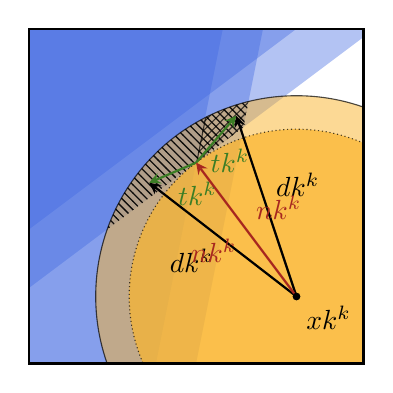
\begin{tikzpicture}[scale=0.85]
                    % Linear constraints
                    \uncover<1,2,6->{\fill[color=RoyalBlue,opacity=0.4] (-4,-1) -- (-1.5,-1) -- (-0.5,4) -- (-4,4) -- cycle;}
                    \uncover<3-5>{\fill[color=RoyalBlue,opacity=0.4] (-4,-1) -- (-2.1,-1) -- (-1.1,4) -- (-4,4) -- cycle;}
                    \uncover<1,2,6>{\fill[color=RoyalBlue,opacity=0.4] (-4,1) -- (0,4) -- (-4,4) -- cycle;}
                    \uncover<3-5,7->{\fill[color=RoyalBlue,opacity=0.4] (-4,0.125) -- (1,3.875) -- (1,4) -- (-4,4) -- cycle;}

                    % Trust regions
                    \begin{scope}
                        \clip (-4,-1) rectangle (1,4);
                        \draw[fill=Dandelion,draw opacity=0.7,fill opacity=0.5] (0,0) circle (3);
                        \draw[densely dotted,fill=Dandelion,opacity=0.7] (0,0) circle (2.5);
                    \end{scope}

                    % Feasible region for the tangential subproblem
                    \begin{scope}
                        \clip (-4,0.125) -- (-1.5,2) -- (-1.1,4) -- (-4,4) -- cycle;
                        \uncover<4-5,10>{\fill[pattern=north west lines,opacity=0.7] (0,0) circle (3);}
                    \end{scope}
                    \begin{scope}
                        \clip (-4,0.125) -- (-27/34,43/17) -- (-0.5,4) -- (-4,4) -- cycle;
                        \uncover<8,9>{\fill[pattern=north west lines,opacity=0.7] (0,0) circle (3);}
                    \end{scope}
                    \begin{scope}
                        \clip (-1.5,2) -- (-1.1,4) -- (-0.5,4) -- (-27/34,43/17) -- cycle;
                        \uncover<10>{
                            \fill[pattern=crosshatch,opacity=0.7] (0,0) circle (3);
                            \draw[thick,opacity=0.7] (-1.5,2) -- (-1.365785,2.671073);
                            }
                    \end{scope}

                    % Frame and annotations
                    \uncover<5>{
                        \draw[-stealth,thick,OliveGreen] (-1.5,2) -- (-2.2,1.7);
                        \node[below,xshift=9pt,text=OliveGreen] at (-1.85,1.85) {$\tstep[k]$};
                        \draw[-stealth,thick] (0,0) -- (-2.2,1.7);
                        \node[below left] at (-1.1,0.85) {$\step[k]$};
                    }
                    \uncover<9>{
                        \draw[-stealth,thick,OliveGreen] (-1.5,2) -- (-0.9,2.7);
                        \node[below,xshift=5pt,text=OliveGreen] at (-1.2,2.35) {$\tstep[k]$};
                        \draw[-stealth,thick] (0,0) -- (-0.9,2.7);
                        \node[above right] at (-0.45,1.35) {$\step[k]$};
                    }
                    \uncover<2->{\draw[-stealth,thick,Mahogany] (0,0) -- (-1.5,2);}
                    \uncover<2-5>{\node[above right,text=Mahogany] at (-0.75,1) {$\nstep[k]$};}
                    \uncover<6->{\node[below left,text=Mahogany] at (-0.75,1) {$\nstep[k]$};}
                    \draw[fill] (0,0) circle (1.4pt) node[below right] {$\iter[k]$};
                    \draw[thick] (-4,-1) rectangle (1,4);
                \end{tikzpicture}
            \end{center}
        \end{column}
        \begin{column}{0.55\textwidth}
        \end{column}
    \end{columns}

    \begin{itemize}
        \item Classical approach of \textcite{Conn_Gould_Toint_2000}.
    \end{itemize}
\end{frame}

\section{Interpolation-based models}

\begin{frame}{Interpolation-based quadratic models}
    \begin{itemize}
        \item Models of \textcite{Powell_2004b}.
        \item Least $H^2$-norm updating models of Xie and Yuan.
    \end{itemize}
\end{frame}

\begin{frame}{Updating the interpolation set}
    To do.
\end{frame}

\section{Gap between theory and practice}

\begin{frame}{A lot of questions must be addressed}
    To do.
\end{frame}

\section{Implementation and experiments}

\begin{frame}{The Python implementation of COBYQA}
    \begin{columns}
        \begin{column}{0.5\textwidth}
            \begin{center}
                \qrcode{https://www.cobyqa.com/}\\[1ex]
                \href{https://www.cobyqa.com/}{Documentation}
            \end{center}
        \end{column}
        \begin{column}{0.5\textwidth}
            \begin{center}
                \qrcode{https://github.com/cobyqa/cobyqa/}\\[1ex]
                \href{https://github.com/cobyqa/cobyqa/}{Source code}
            \end{center}
        \end{column}
    \end{columns}
\end{frame}

\begin{frame}{Comparing COBYQA with existing DFO solvers}
    To do.
\end{frame}

\begin{frame}{Performance on bound-constrained problems}
    To do.
\end{frame}

\begin{frame}{Performance on nonlinearly constrained problems}
    To do.
\end{frame}

\begin{frame}{Comparison with COBYLA}
    To do.
\end{frame}

\section{Conclusion}

\begin{frame}{Conclusion and future work}
    To do.
\end{frame}

\appendix

\begin{frame}[t,allowframebreaks]{References}
    \printbibliography[heading=none]
\end{frame}

\end{document}
